\chapter{绪论}
\section{背景及意义}
\label{sec:env}

\subsection{背景}
%\footnote{参考自\url{https://blog.csdn.net/kk1125778230/article/details/129017176}}
如果要谈Linux是从哪里来,是怎么来的,那就还得从Unix操作系统说起。1968
年贝尔实验室、麻省理工、通用电器公司的研究人员开发了名叫“多路复用信息
和计算机系统”简称Multics的特殊操作系统,Mutics是在二战结束后的冷战时期
诞生的,1957年苏联发射了第一颗人造卫星,进而准备发射载人宇宙飞船;美国
航天局的研究这时却连连受挫,美国总统埃森豪威尔便下决心发展科技,巨款支
持科学界。科学家们开始设想将大型计算机作为一种公共设施,通过许许多多的
终端为用户提供计算时间的“计算机公用事业”,但是最终以失败告终。

1969年,贝尔实验室的Ken Thompson和Dennis Ritchie为了把名叫太空旅行的游
戏移植到一台没人用的PDP-7小型机上,给程序中加入了文件管理、进程管理的功
能,和一组实用工具,一个只能给2个用户使用的系统诞生了。受到MULTICS的影
响,Brian Kernighan玩笑地给系统取名为“UNICS”(没路信息与计算系统),取
谐音便是“UNIX”。1969 --- 1970年,AT\&T的贝尔实验室开发了UINX系统,引起了
众人的关注,很多人找Thompson和Ritchie要Unix的源代码。一份份的Unix源码被
流传到各个实验室、学校、公司。

后来AT\&T 回收了Unix版权,特别是要求禁止对学生群体提供Unix 系统源代码,
这引起了人们的恐慌。于是在1984年,Richand Stallman 发起了开发自由软件
的运动。一名大学教授为了教学使用开发了Minux,因为Minux操作系统主要用于
教学使用,所以不适合商用。后来赫尔辛基大学的一名学生名叫Linus Torvalds,
接触了Unix,发现Unix操作等待时间长等一些问题,因而学习了Minux的核心技
术,开发了Linux。1991年底,Linus Torvalds 公开了Linux 内核源码0.02 版,
并吸引了世界各地的顶级黑客不断的完善Linux,一直发展的到今天。Linux是一
种自由和开放源代码的类UNIX操作系统,严格来讲,Linux只是操作系统内核本
身,但通常采用“Linux内核”来表达该意思,而Linux则常用来指基于Linux内核的完整操作系统。

\subsection{意义}

随着IT行业的高速发展,现在基本上每家每户都会使用计算机,而想正常的使用
计算机来处理一些事情,比如办公、通信、游戏娱乐等,都得有支持应用软件运
行的一个“载具”,而这个“载具”就是操作系统。
操作系统,如图\ref{fig:os}所示,是硬件基础上的第一层软件,是用户进程与
计算机硬件之间的桥梁,它能有效管理软硬件资源,合理组织工作流程,向用户
进程提供服务,使用户能够更方便地使用计算机,使整个计算机系统能高效运行,
可以说是计算机软件系统的“心脏”。

\begin{figure}
  \centering
  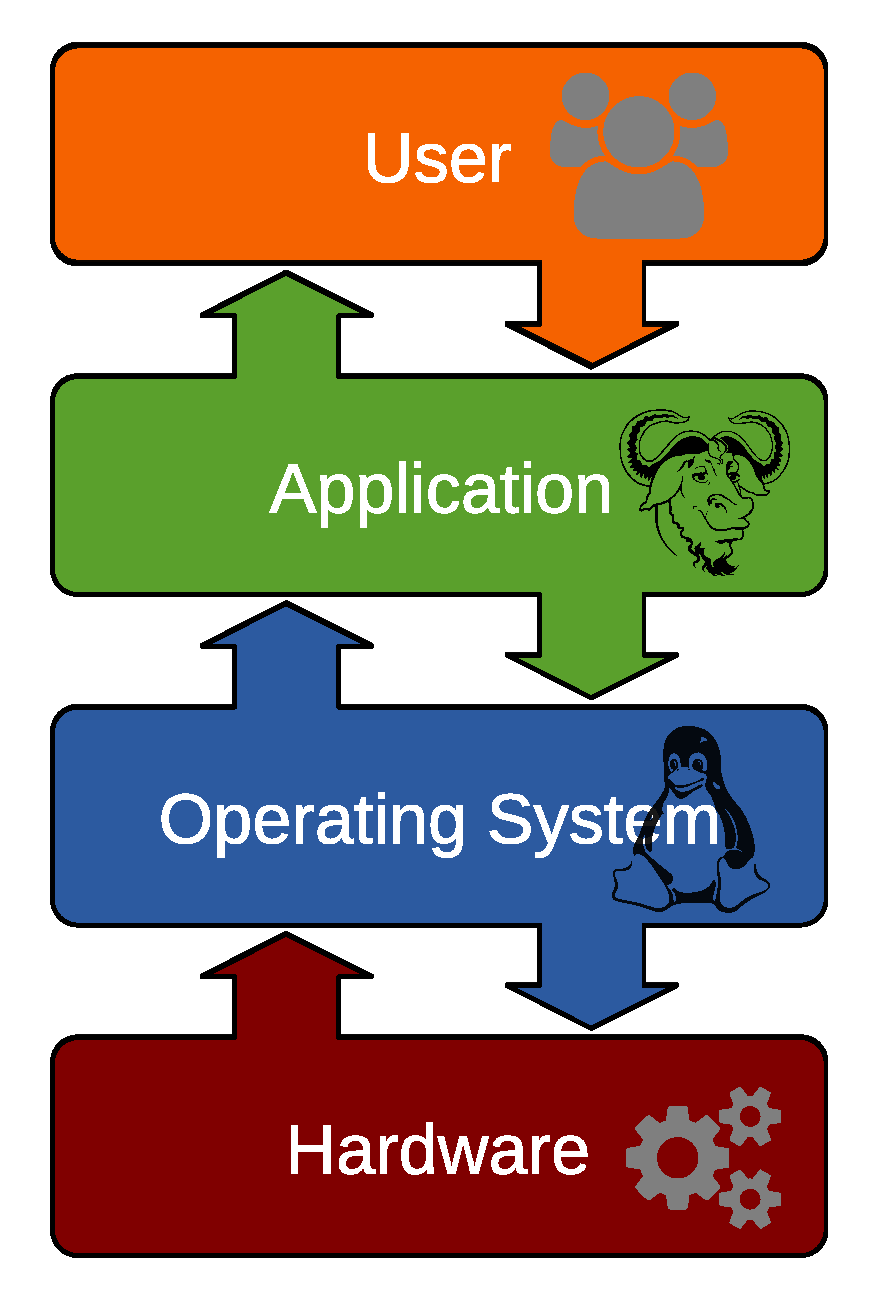
\includegraphics[width=.3\linewidth]{os}
  \caption{操作系统是介于用户进程和硬件之间的软件}
  \label{fig:os}
\end{figure}

现在市面上最流行的操作系统莫过于Windows和Linux。大多数人都是从Windows系
统开始了解计算机和网络的,Windows易用性高,很适合新接触计算机的人上手,
但也因此使多数人对操作系统的选择上产生了很大的误区,认为Windows系统
比Linux系统好用且简单。对于那些使用计算机只是为了上个网看个视频、打打游
戏、查查资料的用户确实使用Windows系统是最简单的。但抛开这些不
谈,Linux是使用命令行字符模式为主要操作方式,而Windows是使用窗口、图标、
鼠标点击形象化的方式为主要操作方式,从这点来看Windows系统就得比Linux系
统要多耗费更多的计算机内存,并且“鼠标+键盘”的操作效率比起使用键盘敲指令
就可以完成操作的效率是要慢很多的。甚至熟练后Linux系统的查资料、看视频等
体验都是要优于Windows系统的。这些只是用户基本体验上的区别,
而Linux与Windows最大的不同在于Linux系统是自由的。自由,不止是说使用这个
系统不出钱,重点是Linux内核是完全开源的,如果本身技术水平比较高的话,甚
至可以用它自己DIY一个只属于自己的任何风格的OS,仔细一想这不是一件非常酷
且很有意思的事吗?而Windows系统的内核是闭源的,所以到现在Linux的版本有
很多很多,而Windows仅仅只有微软公司的Windows XP、Win7、Win11等,用户的
选择很有限。除版本区别外,Linux与Windows还有个很大的区别在于安全性,因
为Linux的软件基本上也都是开源的,在这个大家庭里的很多都是相互扶持的关系,
互帮互助,你需要什么都可以通过一个指令直接获取到软件包直接安装到你的电
脑上。而Windows系统想要个软件,如果不是官方的可能还要担心有没有病毒等,
若是官方的也有可能需要收费购买,破解版又缺乏了安全性并且也是不合法
的\cite{lt2021}。

综上所述,所以我觉得研究并且能够做出一个属于自己的基于Linux技术的OS是
一件很有意义的事,它不但能够令我对Linux的运行逻辑更加清晰,
也能够使我对操作系统开发的了解更加深入透彻。

\section{开发工具及环境}

\subsection{开发工具}

\begin{description}
\item[编辑器:] VIM v0.7.2; Emacs v28.2;
\item[编译器:] GCC v12.2.0;
\item[汇编器:] NASM v2.16.01;
\item[虚拟机:] Bochs v2.6.9\footnote{宿主机如果是Debian GNU/linux可以直
    接敲命令:“sudo apt install vgabios bochs bochs-x bximage”来安
    装bochs。};
\item[Makefile:] GNU Make v4.3.
\end{description}

\subsection{环境配置}

\begin{description}
\item[宿主OS:] Linux v6.1.0-7-amd64 \#1 SMP Debian v6.1.20-2
\item[硬件:] x86\_64
\end{description}

\section{该研究的主要内容}

该研究的主要内容为从操作系统最底层的原理探索一个操作系统从0到1的实现。首先是计算机的
开机过程:引领我们走向计算机这一整个系统的神秘代码,\texttt{0x7C00},一切都要从它开始。计
算机通电开机之后,BIOS便会开始自检,在找到可用的磁盘后,BIOS就会把它的第一个扇区加载到
\texttt{0x7C00},之后由一个512字节的主引导记录MBR\footnote{实际上只有446字节用于引导程序和参数,剩
  下的64字节用于分区表和2字节用于结束标记的\texttt{0x55}和
  \texttt{0xAA}。}从BIOS中接过系统的控制权,也就是CPU的使用权。MBR便是从
\texttt{0x7C00}处接管CPU的,刚好是512字节。之后,MBR寻找操作系统所在的
分区,我们规定用\texttt{0x80}来表示分区上有引导程序,方便MBR从众多分区
中方找到操作系统所在的分区,MBR如果找到了这个分区,就会将CPU使用权交给
这个分区上的引导程序,该引导程序通常就是内核加载器,所以,为了让MBR能
够更方便的在那么大的分区里找到内核加载器,通常会把内核加载器的入口
地址固定在分区最开始的扇区,该扇区就是操作系统引导扇区(MBR
扇区)。而在MBR扇区的前3个字节处存放了跳转指令,目的是为了让MBR找到分
区交接工作后,将处理器带入操作系统引导程序中,至此MBR就完成了所有工作,
CPU的控制权就交到了内核手里。到此为止,计算机也只算是开机了而已,此时计算机的状态就像是在执行代码:
\begin{codeblock}
\begin{ccode}
while(1)
{
  操作系统代码();
}
\end{ccode}  
\end{codeblock}

因此,想让计算机知道我们要让它做什么事就还得需要进程,当然,
一个进程也
只能完成一项工作,在很多时候工作往往并不简单,因此,我们想让进程尽可能的同时多做一些子工作,
而这些“子工作”就是线程。现在有了进程以及线程,但是计算机仍然在做一个\texttt{while(1)}的循
环,所以还需要给计算机一个中断,让它能够判断出事情的重要程度,也就是优
先级,来选择先把哪件事情
给做好,之后再进行之前没完成的工作,到这才算是实现了一个操作系统\cite{yy2009}。


%%% Local Variables:
%%% mode: latex
%%% TeX-master: "../thesis"
%%% End:
